\documentclass[14pt]{extarticle} 
\usepackage{amsmath,mathtools,amsfonts,amsthm,amssymb,hyperref,tikz}
\usepackage{wasysym,geometry,bussproofs,latexsym,parskip,bookmark}
\newtheorem{defn}{Definition}
\newtheorem{thm}{Theorem}
\newtheorem{claim}{Claim}
\newtheorem{lemma}{Lemma}
\hypersetup{colorlinks,allcolors=blue,linktoc=all}
\geometry{a4paper} 
\geometry{margin=0.5in}
\title{Math for CS 2015/2019 Problem Set 8 solutions}
\author{https://github.com/spamegg1}
\begin{document}
\maketitle
\tableofcontents

\section{Problem 1}
Prove Corollary 11.10.12: If all edges in a finite weighted graph have distinct weights, then the graph has a unique MST in the course textbook.

{\it Hint:} Suppose $M$ and $N$ were different MST’s of the same graph. Let $e$ be the smallest edge in one and not the other, say $e \in M - N$, and observe that $N + e$ must have a cycle.
\begin{proof}
First let's clarify: when we are talking about MST's, the graph $G$ is always finite, connected, edge-weighted and undirected, and the edge weights are always positive (even though the textbook does not make this clear due to its informal conversational style of writing).

Let's follow the hint, and the proof of Lemma 11.10.11. Recall the notation $w(e)$ to denote the edge weight of an edge $e$.

1. Assume $G$ is a finite weighted graph with all edges having distinct positive weights.

2. Argue by contradiction and assume $G$ has two different MST's, $M$ and $N$. Notice that $w(M) = w(N)$, since they are both MST's of the same graph $G$.

3. Since $M$ and $N$ are different, there exists an edge that belongs to one of them but not both. So $(M-N) \cup (N-M)$ is nonempty. 

4. Let $e$ be the edge in $(M-N) \cup (N-M)$ with the (strictly) smallest weight ($e$ exists because all edges have distinct weights). We don't know if $e \in M-N$ or $e \in N-M$, but these two cases have similar proofs, so without loss of generality, assume $e \in M-N$.

5. Say $e$ is the edge between the two nodes $a$ and $b$. Since $N$ is a spanning tree, there is a path $p$ in $N$ between the nodes $a$ and $b$.

6. Since $e$ is not in $N$, $e$ is not part of the path $p$. So $N + e$ contains a cycle that starts and ends at $a$. (The path $p$ starts at $a$ and ends at $b$, then $e$ connects $b$ to $a$, completing the cycle.)

7. Since $e \in M$, if all the edges on the path $p$ belonged to $M$, then $M$ would contain the cycle $p + e$, contradicting the fact that $M$ is a tree. So there is an edge $g$ on the path $p$ such that $g \in N-M$.

8. By (4) we have $w(e) < w(g)$. So we have
$$
w(N + e - g) = w(N) + w(e) - w(g) < w(N)
$$

9. Then $N + e - g$ is also a spanning tree, and its weight is strictly smaller than $W(N)$ which is a contradiction to the minimality of $N$.

10. So our initial assumption in (2) was false, and $G$ has a unique MST.
\end{proof}

\section{Problem 2}
A basic example of a simple graph with chromatic number $n$ is the complete graph on $n$ vertices, that is $\chi (K_n) = n$. This implies that any graph with $K_n$ as a subgraph must have chromatic number at least $n$. It’s a common misconception to think that, conversely, graphs with high chromatic number must contain a large complete subgraph. In this problem we exhibit a simple example countering this misconception, namely a graph with chromatic number four that contains no {\it triangle} (length three cycle) and hence no subgraph isomorphic to $K_n$ for $n \geq 3$. Namely, let $G$ be the 11-vertex graph of Figure 1. The reader can verify that $G$ is triangle-free.
\begin{center}
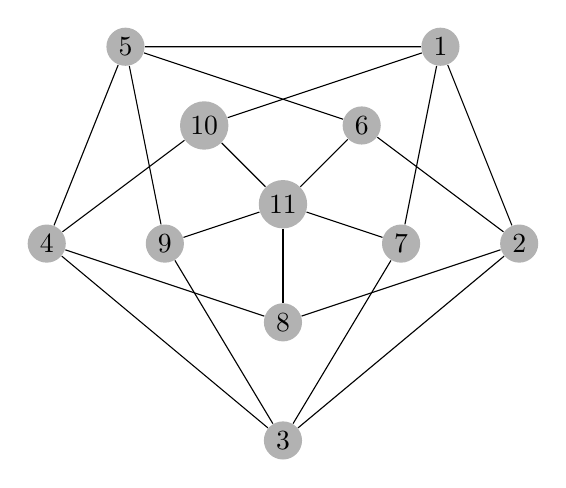
\begin{tikzpicture}
\tikzstyle{vertex}=[circle,fill=black!30,minimum size=12pt,inner sep=2pt]
\node[vertex] (G_1) at (2,2)    {1};
\node[vertex] (G_2) at (3,-0.5) {2};
\node[vertex] (G_3) at (0,-3)   {3};
\node[vertex] (G_4) at (-3,-0.5){4};
\node[vertex] (G_5) at (-2,2)   {5};
\node[vertex] (G_6) at (1,1)  {6};
\node[vertex] (G_7) at (1.5,-0.5) {7};
\node[vertex] (G_8) at (0,-1.5)   {8};
\node[vertex] (G_9) at (-1.5,-0.5)  {9};
\node[vertex] (G_{10}) at (-1,1) {10};
\node[vertex] (G_{11}) at (0,0)   {11};
\draw (G_1) -- (G_2) -- (G_3) -- (G_4) -- (G_5) -- (G_1) --cycle;
\draw (G_{11}) -- (G_6);
\draw (G_{11}) -- (G_7);
\draw (G_{11}) -- (G_8);
\draw (G_{11}) -- (G_9);
\draw (G_{11}) -- (G_{10});
\draw (G_1) -- (G_7);
\draw (G_1) -- (G_{10});
\draw (G_2) -- (G_6);
\draw (G_2) -- (G_8);
\draw (G_3) -- (G_7);
\draw (G_3) -- (G_9);
\draw (G_4) -- (G_8);
\draw (G_4) -- (G_{10});
\draw (G_5) -- (G_6);
\draw (G_5) -- (G_9);
\end{tikzpicture}
\end{center}
\subsection{(a)}
Show that $G$ is 4-colorable.
\begin{proof}
Proof by picture:
\begin{center}
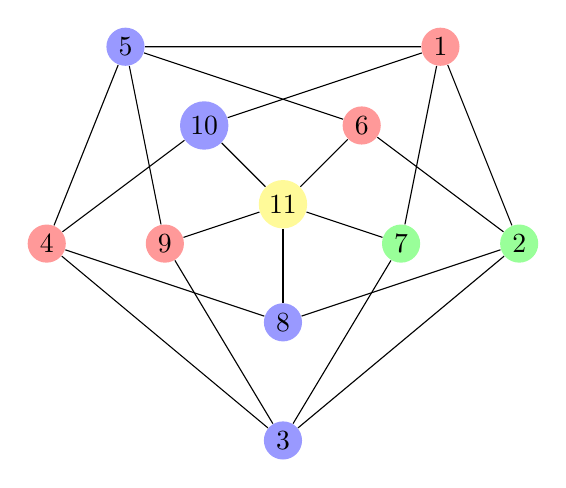
\begin{tikzpicture}
\tikzstyle{blue}=[circle,fill=blue!40,minimum size=12pt,inner sep=2pt]
\tikzstyle{red}=[circle,fill=red!40,minimum size=12pt,inner sep=2pt]
\tikzstyle{green}=[circle,fill=green!40,minimum size=12pt,inner sep=2pt]
\tikzstyle{yellow}=[circle,fill=yellow!40,minimum size=12pt,inner sep=2pt]
\node[red] (G_1) at (2,2)    {1};
\node[green] (G_2) at (3,-0.5) {2};
\node[blue] (G_3) at (0,-3)   {3};
\node[red] (G_4) at (-3,-0.5){4};
\node[blue] (G_5) at (-2,2)   {5};
\node[red] (G_6) at (1,1)  {6};
\node[green] (G_7) at (1.5,-0.5) {7};
\node[blue] (G_8) at (0,-1.5)   {8};
\node[red] (G_9) at (-1.5,-0.5)  {9};
\node[blue] (G_{10}) at (-1,1) {10};
\node[yellow] (G_{11}) at (0,0)   {11};
\draw (G_1) -- (G_2) -- (G_3) -- (G_4) -- (G_5) -- (G_1) --cycle;
\draw (G_{11}) -- (G_6);
\draw (G_{11}) -- (G_7);
\draw (G_{11}) -- (G_8);
\draw (G_{11}) -- (G_9);
\draw (G_{11}) -- (G_{10});
\draw (G_1) -- (G_7);
\draw (G_1) -- (G_{10});
\draw (G_2) -- (G_6);
\draw (G_2) -- (G_8);
\draw (G_3) -- (G_7);
\draw (G_3) -- (G_9);
\draw (G_4) -- (G_8);
\draw (G_4) -- (G_{10});
\draw (G_5) -- (G_6);
\draw (G_5) -- (G_9);
\end{tikzpicture}
\end{center}
\end{proof}
\subsection{(b)}
Prove that $G$ can't be colored with 3 colors.
\begin{proof}
1. Argue by contradiction and assume $G$ is colored with 3 colors (say Red, Green, Blue).

2. Nodes 1,2,3,4,5 form a 5-cycle. This forces all 3 colors to be used: two of the colors twice, and the other color once. 

3. Without loss of generality, assume that the color that is only used once on 1,2,3,4,5 is R (red), and without loss of generality, assume the node that gets colored R is 1. So 2,3,4,5 are colored G or B.

4. Notice that nodes 2,3,4,5,6 also form a 5-cycle. So by (3), node 6 must also be colored R.

5. Since node 1 is connected to nodes 7 and 10, and node 1 is R, nodes 7 and 10 must be G or B.

6. By (4) and (5), nodes 6, 7, 10 all have different colors. But they are all connected to node 11, which has the same color as one of them! Contradiction.

7. So $G$ is not 3-colorable.
\end{proof}

\section{Problem 3}
The preferences among 4 boys and 4 girls are partially specified in the following table:
$$
\begin{array}{|c c c c c|}
\hline
B1: & G1 & G2 & - & - \\
B2: & G2 & G1 & - & - \\
B3: & - & - & G4 & G3 \\
B4: & - & - & G3 & G4 \\
\hline 
G1: & B2 & B1 & - & - \\
G2: & B1 & B2 & - & - \\
G3: & - & - & B3 & B4 \\
G4: & - & - & B4 & B3 \\
\hline 
\end{array}
$$
\subsection{(a)}
Verify that
$$
(B1, G1), (B2, G2), (B3, G3), (B4, G4)
$$
will be a stable matching whatever the unspecified preferences may be.
\begin{proof}
1. Argue by contradiction and assume there is a way to specify the remaining preferences that makes the matching unstable.

2. By (1) there is a rogue couple $B, G$ such that $B$ prefers $G$ to his wife and $G$ prefers $B$ to her husband.

3. Case 1: $B = B1$. In this case $B$ is already married to his top preference $G1$, but by (2) $B$ prefers $G$ to $G1$, contradiction.

4. Case 2: $B = B2$. Similar to Case 1, contradiction.

5. Case 3: $B = B3$. In this case $B$ prefers $G1, G2$ to his wife $G3$, so $G = G1$ or $G = G2$. But $G1, G2$ both prefer their husbands $B1, B2$ over $B3$, contradiction.

6. Case 4: $B = B4$. Similar to Case 3, contradiction.

7. So our assumption in (1) was false, and this is a stable matching.

\end{proof}
\subsection{(b)}
Explain why the stable matching above is neither boy-optimal nor boy-pessimal and so will not be an outcome of the Mating Ritual.
\begin{proof}
1. Both $B1$ and $B2$ are married to their top preferences, so the stable matching is not boy-pessimal.

2. Both $B3$ and $B4$ are married to their bottom preferences, so the stable matching is not boy-optimal. 

3. Theorem 11.6.10 says that the Mating Ritual results in a boy-optimal stable matching, so this cannot be the result of the Mating Ritual.
\end{proof}
\subsection{(c)}
Describe how to define a set of marriage preferences among $n$ boys and $n$ girls which have at least $2^{n/2}$ stable assignments.

{\it Hint:} Arrange the boys into a list of $n/2$ pairs, and likewise arrange the girls into a list of $n/2$ pairs of girls. Choose preferences so that the $k$th pair of boys ranks the $k$th pair of girls just below the previous pairs of girls, and likewise for the $k$th pair of girls. Within the $k$th pairs, make sure each boy’s first choice girl in the pair prefers the other boy in the pair.
\begin{proof}
1. We are given $n$ boys $B1, \ldots, Bn$ and $n$ girls $G1, \ldots, Gn$. For simplicity assume $n$ is even, so that $n/2$ is an integer.

2. Define preferences as follows. It's similar to part (a) but generalized to $n$ boys and $n$ girls. 

There are two possibilities for each boy pair and each girl pair. For $1 \leq k \leq n/2$, the $2k-1$th and $2k$th preferences of boys $B(2k-1)$ and $B(2k)$ are girls $G(2k-1)$ and $G(2k)$, but they prefer these girls in reverse order of each other. Then the preferences of the girls $G(2k-1)$ and $G(2k)$ mirror them. The remaining preferences are left undefined.

For example, $B1$, $B2$, $G1$ and $G2$'s top two preferences in order are:

either $B1: G1, G2$; $B2: G2, G1$; $G1: B1, B2$; and $G2: B2, B1$,

or $B1: G2, G1$; $B2: G1, G2$; $G1: B2, B1$; and $G2: B1, B2$.

Then, similar for all the other pairs too:
$$
\begin{array}{|c c c c c c|}
\hline
B1: & G1 \text{ or } G2 & G2 \text{ or } G1 & ... & - & - \\
B2: & G2 \text{ or } G1 & G1 \text{ or } G2 & ... & - & - \\
... & ... & ... & ... & ... & ... \\
B(n-1): & - & - & ... & G(n-1) \text{ or } Gn & Gn \text{ or } G(n-1) \\
Bn: & - & - & ... & Gn \text{ or } G(n-1) & G(n-1) \text{ or } Gn \\
\hline
G1: & B1 \text{ or } B2 & B2 \text{ or } B1 & ... & - & - \\
G2: & B2 \text{ or } B1 & B1 \text{ or } B2 & ... & - & - \\
... & ... & ... & ... & ... & ... \\
G(n-1): & - & - & ... & B(n-1) \text{ or } Bn & Bn \text{ or } B(n-1) \\
Gn: & - & - & ... & Bn \text{ or } B(n-1) & B(n-1) \text{ or } Bn \\
\hline 
\end{array}
$$

3. We can generalize the argument given in part (a), by induction on the number of pairs, to prove that no matter what the unspecified preferences are, these preferences give a stable matching. (Please do that! I'm too tired.)

4. Since there are $n/2$ pairs, and for each pair there are 2 choices of preferences, there are $2^{n/2}$ different ways to set these preferences. By (3) each one of these preferences lead to a stable matching. So there are at least $2^{n/2}$ stable matchings.
\end{proof}






























\end{document}